\documentclass[cn,10pt,math=newtx,chinesefont=founder]{../elegantbook}

\title{物理人才培育計畫考古題}
\subtitle{2021年}

\author{李宥頡}
\institute{National Taiwan University}
\setcounter{tocdepth}{3}

%\logo{logo-blue.png}
\cover{cover.jpg}

% 本文档命令
\usepackage{array}
\newcommand{\ccr}[1]{\makecell{{\color{#1}\rule{1cm}{1cm}}}}

\definecolor{customcolor}{RGB}{32,178,170}
\colorlet{coverlinecolor}{customcolor}

\begin{document}

\maketitle

\mainmatter

\chapter{數學複習}
\section{三角函數}
\newpage
\section{向量}
\newpage
\section{微積分}
\newpage
\chapter{力學}

\section{直線運動與平面運動}
\subsection{重點整理}
\newpage
\subsection{考古題練習}
\begin{example}
    有一人騎著自行車由靜止以 $0.10$ 公尺/秒 $^{2}$ 之等加速度加速前進 60 秒後就維持等速前進,
    再騎了 5 分鐘後,他便以-0.05 公尺/秒 $^{2}$ 之等加速度行進,直到車停下來。請問:
    \begin{enumerate}[label=(\alph*)]
        \item 他共騎了多少時間
        \item 他共騎了多少公尺
    \end{enumerate}
\end{example}
\begin{solution}
\end{solution}
\vspace{7cm}



\begin{example}
    有一物體在 $t=0$ 時由靜止從原點沿著 $x$-軸運動, 其位置對時間的關係如圖 示 $\circ$ 請問在 $t=6 \mathrm{~s}$ 時該物體的速度為 $\_\_\_$ , 所受到的加速度為 $\_\_\_$ 。
\end{example}
\begin{solution}
    
\end{solution}
\begin{figure}[htbp]
    \flushright
    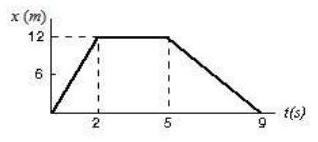
\includegraphics[width=0.3\textwidth]{image/1.jpeg}
\end{figure}
\vspace{6cm}



\begin{example}
    某人將一質量為 $m$ 的高爾夫球以和地面的夾角為 $\theta, v_{0}$ 的初速擊出。不考慮空氣阻力 , 該球可以到達的最大高度為$\_\_\_$ ; 該球在空中停留的時間 $\_\_\_$ 。 (重力加速度為 $g$ )
\end{example}
\begin{solution}
    
\end{solution}
\newpage


\section{靜力平衡}
\subsection{重點整理}
\newpage
\subsection{考古題練習}
\begin{example}
    將一質量為 $10.0$ 公斤鋁梯靠在一垂直之平滑牆壁上。梯子與牆壁之間的夾角 為30度 , 梯子的長度為3.10公尺。有一工人站在離鋁梯地面端1.50公尺的鋁 梯横桿上,該工人的質量為 $60.0$ 公斤。如果該鋁梯不滑動,地面跟鋁梯之間 的摩擦力是多少牛頓? $\_\_\_$ (請忽略鋁梯與牆壁之間的磨擦力)如果鋁梯和地 面之間的靜摩擦係數 $\mu_{\mathrm{k}}=0.31$, 請問該鋁梯是否會滑動? $\_\_\_$ $\left(\cos 30^{\circ}=\sqrt{3} / 2\right.$; $\left.\sin 30^{\circ}=1 / 2\right)$ 
\end{example}
\begin{solution}

\end{solution}
\begin{note}
\end{note}
\newpage

\begin{example}
    有一艘潛艇長為110公尺,船體的直徑是10公尺。假設潛艇的上方是平坦 的,其面積為 1,100 平方公尺。當潛艇在水面下250公尺時,海水作用在潛艇上方的力為 $\_\_\_$ 牛頓。(海水密度1,024公斤 /立方公尺)
\end{example}
\begin{solution}

\end{solution}
\vspace{6cm}
\begin{example}
    物體在運動時所受到空氣的阻力的大小可表示為 $F_{\mathrm{D}}=\mathrm{Dv}^{2}$, 其中 $\mathrm{D}$ 為一常數 (和物體的截面積以及空氣的密度有關)。今有甲乙兩顆體積相同之圓球形物體從高空落下,在落地之前皆達到終端速度 。甲的質量是乙的質量之 4 倍 在著地之瞬間,物體甲之速率為物體乙速率之$\_\_\_$倍。
\end{example}
\begin{solution}
\end{solution}
\newpage


%功能
\section{功能}
\subsection{重點整理}
\newpage
\subsection{考古題練習}
\begin{example}
    一質量為 1000 公斤 ,初速為 $20.0$ 公尺/秒之汽車受到一定值之摩擦力而開始 減速 , 
    經過 100 公尺後該車完全停止。該車所受到之摩擦力為$\_\_\_$牛頓。 如果此摩擦力完全來自地面與輪胎間之摩擦力,則地面與輪胎間之動摩擦係數為$\_\_\_$。
\end{example}
\begin{solution}
    
\end{solution}
\vspace{6cm}
\begin{example}
    某人用板手要將一螺絲旋緊在水平桌面上 , 該螺絲之螺帽之直徑為 $0.860$ 公 分。他總共轉了 $30.5$ 圈才完成。假設在旋緊過程中,桌子和螺絲之摩擦力為 定值( $14.5$ 牛頓), 請問將該螺絲旋緊鎖需要做的功為 $\_\_\_$ 焦耳。
\end{example}
\begin{solution}

\end{solution}
\vspace{6cm}

\begin{example}
    墨西哥灣流是全球最大的洋流(在大西洋) , 我們假設它的截面是寬度 100 公 里,深度 500 公尺的長方形 $^{\circ}$ 洋流的流速為 $2.0$ 公尺/秒 , 洋流的溫度高出周 遭海水 $5^{\circ} \mathrm{C}$ 。請算出此洋流作用在大西洋的功率為$\_\_\_$ 瓦特。(水的比熱為 $\left.4,186 \mathrm{~J} / \mathrm{kg}-{ }^{\circ} \mathrm{C}\right)$
\end{example}
\begin{solution}

\end{solution}
\vspace{6cm}

\begin{example}
     已知在某地區接受到日光平均強度為 100 瓦/平方公尺 , 平均每天日照時間 6 小時,而太陽能板可將 $20 \%$ 的太陽能轉換成電能。若某戶住家平均每天耗電為 12 度電,則需裝設$\_\_\_$平方公尺的太陽能板,方可自給自足。
\end{example}
\begin{solution}
    
\end{solution}
\vspace{6cm}
\section{圓周運動}
\subsection{重點整理}
\newpage
\subsection{考古題練習}
\begin{example}
    一繩子的一端綁著一顆質量為 $m$ 的石頭並將該石頭在垂直方向作圓周運動 (半徑為 $R)$ 。如果當石頭在最低點時,繩子所受到的張力是石頭重量的 5 倍。 則石頭在該點的速率為$\_\_\_$, 當石頭在最高為點的速率為$\_\_\_$(繩子之質量可以忽略)
\end{example}
\begin{solution}
    
\end{solution}
\vspace{6cm}
%萬有引力
\section{萬有引力}
\subsection{重點整理}
\newpage
\subsection{考古題練習}
\begin{example}
    火星的質量是 $6.4 \times 10^{23}$ 公斤 ,和地球之間的最短距離為 $5.6 \times 10^{14}$ 公尺 。在這 個時候一輛為16,000公斤的卡車距離你多少公尺時,卡車對你造成的重力大小會等於火星對你所造成的重力?答案:$\_\_\_$ 公尺。
\end{example}
\begin{solution}

\end{solution}
\vspace{6cm}
\begin{example}
    一行星的質量為地球之兩倍, 半徑為地球之 $1.5$ 倍。在該行星表面的重力加速度 $\mathrm{g}$ 之值為$\_\_\_$公尺/秒 $^{2}$ 。
\end{example}
\begin{solution}
\end{solution}
\vspace{6cm}

\begin{example}
    地球的質量是 $5.97 \times 10^{24}$ 公斤 , 月球的質量為 $7.36 \times 10^{22}$ 公斤 ,月球繞地球的軌道距離地心 384,000 公里。請問地球-月球系統的質量中心距離地心多少公里 ? (請注意有效位數)答案:$\_\_\_$ 公里。
\end{example}
\begin{solution}
    
\end{solution}
\vspace{6cm}
%圓周運動
\begin{example}
    福衛七號衛星的任務軌道高度約為 550 公里, 求衛星繞行地球一周所需要的時間為多久: $\_\_\_$ $^{\circ}$ (地球的半徑為 $6380 \mathrm{~km}$; 地球表面 $g=9.8 \mathrm{~m} / \mathrm{s}^{2}$ )
\end{example}
\begin{solution}

\end{solution}
\vspace{6cm}
\section{簡諧運動}
\subsection{重點整理}
\newpage
\subsection{考古題練習}
\begin{example}
    一彈性係數為 $\mathrm{k}=50$ 牛頓/公尺之彈簧,一端固定在牆上,另一端連接一質量 為 $0.50$ 公斤的物體。將該物體拉長至離平衡點(即將該彈簧伸長) $0.12$ 公尺後 將該物體放開。求該物體運動之週期為 $\_\_\_$ 秒, 該物體所受到之加速度之最 大量值為 $\_\_\_$ 公尺/秒 $^{2}$ 。
\end{example}
\begin{solution}

\end{solution}
\vspace{6cm}


\section{動量與衝量}
\subsection{重點整理}
\newpage
\subsection{考古題練習}
\begin{example}
    將一顆蛋裝在一個特別的盒子裡,盒子跟蛋的質量總共是 $0.144$ 公斤 。如果 讓該盒子從 $3.7$ 公尺的高度自由落下,請問盒子從碰到地面到停止(盒子不會再彈起來)至少要多久才不會將蛋打破?(蛋可承受的最大淨力為 $4.42$ 牛頓) 答案:$\_\_\_$ 秒。
\end{example}
\begin{solution}
    
\end{solution}
\vspace{6cm}

\section{碰撞}
\subsection{重點整理}
\newpage
\subsection{考古題練習}

\begin{example}
    一質量為 $2.0$ 公斤 , 速率為 6 公尺/秒之物體與另一靜止之物體做完全彈性碰撞後,速率變為原來速率之 3 分之 1 , 繼續向原來的方向前進。
    請問該靜止 之物體的質量為$\_\_\_$公斤 。碰撞後該原先靜止之物體的動能變為$\_\_\_$焦耳
\end{example}
\begin{solution}
\end{solution}
\vspace{6cm}
\begin{example}
    一質量為1.5公斤之物體與另一靜止之物體做完全非彈性碰撞後,速率變為原來速率之3分之1,繼續向原來的方向前進。請問該靜止之物體的質量為$\_\_\_$ 公斤。
\end{example}
\begin{solution}
    
\end{solution}
\newpage

%熱
\section{熱}
\subsection{重點整理}
\newpage
\subsection{考古題練習}
\begin{example}
    地球表面海洋的面積為 $3.6 \times 10^{8} \mathrm{~km}^{2}$, 平均的深度為 3,700 公尺。一般來說, 水溫在 1,000 公尺深以下䜌化不大(忽略之)。假設全球 1,000 公尺深以內的平 均水溫為 $10.0^{\circ} \mathrm{C}$, 請計算出如果平均水溫上升 $1.0^{\circ} \mathrm{C}$, 海平面將上升多少?
    答案: $\_\_\_$ $^{\circ}$ (水在 $10^{\circ} \mathrm{C}$ 的體積膨脹係數為 $87.5 \times 10^{-6}{ }^{\circ} \mathrm{C}^{-1}$ )
\end{example}
\begin{solution}

\end{solution}
\vspace{6cm}
\begin{example}
    60 公斤重的慢跑者在半小時產生 $7.0 \times 10^{5}$ 焦耳的熱,如果這些熱不被移除 , 該慢跑者之體溫將上升多少 ${ }^{\circ} \mathrm{C} ?\left(\right.$ 人體的平均比熱為 3500 焦耳/公斤- ${ }^{\circ} \mathrm{C}$ ) 正確之答案:$\_\_\_$

\end{example}
\begin{solution}

\end{solution}
\vspace{6cm}

\begin{example}
    等溫下,物體之輻射熱跟其表面積成正比。有一實心圓柱,其長度為其半徑 之 20 倍。若欲在相同溫度下使其幅射熱變成原來之兩倍,須將該圓柱切成 $\_\_\_$ 塊相同長度之小圓柱。
\end{example}
\begin{solution}

\end{solution}
\vspace{6cm}

\begin{example}
    有一實心圓柱,其長度為其半徑之 12 倍。若欲在相同溫度下使其輻射熱變成原來之兩倍 , 須將該圓柱切成$\_\_\_$塊相同長度之小圓柱。
\end{example}
\begin{solution}
    
\end{solution}
\vspace{6cm}

\begin{example}
    以一加熱器加熱 800 克的純水,升高 $20^{\circ} \mathrm{C}$ 費時 40 秒;而加熱 400 克的某液 體時,升高 $10^{\circ} \mathrm{C}$ 費時 20 秒, 則該液體的比熱為$\_\_\_$卡/克 ${ }^{\circ} \mathrm{C} ; 400$ 克該液體的熱容量為$\_\_\_$卡 $/{ }^{\circ} \mathrm{C}$
\end{example}
\begin{solution}
    
\end{solution}
\newpage
%波
\section{波}
\subsection{重點整理}
\newpage
\subsection{考古題練習}
\begin{example}
    一般人的耳朵可以聼到聲音的頻率為 $20-20,000 \mathrm{~Hz}$,室溫聲速為 343 公尺/秒, 請問人耳可聽到的聲音波長範圍是 $\_\_\_$ 。
\end{example}
\begin{solution}

\end{solution}
\vspace{6cm}
\begin{example}
    高速公路上有一救護車邊行駛邊發出 300 赫茲的警笛聲。救護車的時速為 108 公里, 請寫出在救護車正前方$\_\_\_$和正後方$\_\_\_$測到該警笛聲的波長之值。(聲波在空氣中的傳遞速率為 330 公尺/秒)
\end{example}
\begin{solution}
    
\end{solution}
\vspace{6cm}





\end{document}